\chapter{System Design and Architecture}
\label{chap:architecture}

This chapter presents the architectural design of the Lectura platform through UML diagrams and system schematics, and justifies the technology stack choices through comparative analysis.

\section{Minimum Viable Product (MVP) Scope}
The MVP scope for Lectura was kept deliberately narrow to validate the core idea without unnecessary complexity. The features included in the initial release were: user registration and authentication, multimedia file upload, real-time transcript extraction, automated generation of study artifacts (summaries, quizzes, flashcards, and presentations), and a persistent content library on the frontend. More advanced features such as detailed analytics dashboards and offline synchronization were deferred to future development phases.

\section{System Architecture Overview}
The overall system architecture is documented in Figure~\ref{fig:sys_architecture}. Lectura follows a three-tier architecture: a Client Presentation Layer built with React, an Application Logic Layer implemented in Go, and a Data/Generation Layer consisting of PostgreSQL, Redis, and the Google Gemini API.

\begin{figure}[htbp]
\centering
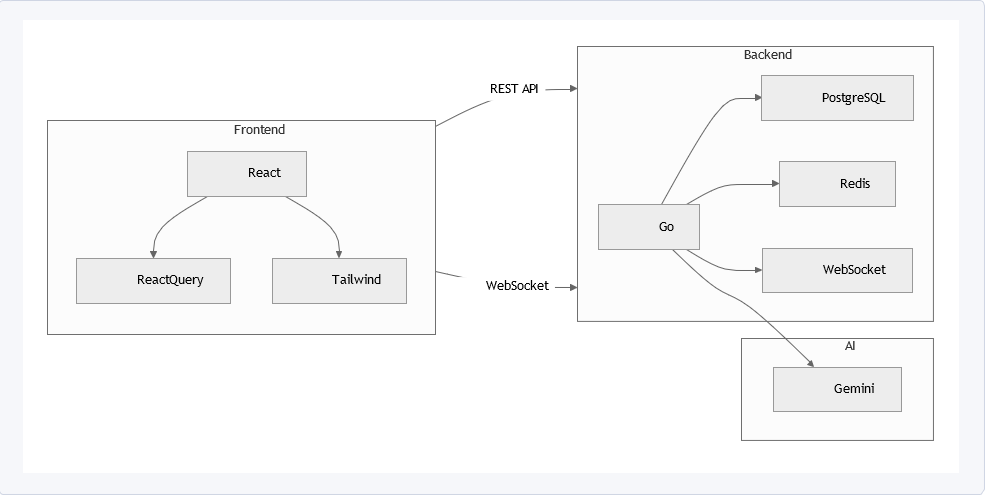
\includegraphics[width=\textwidth]{chapters/chapter05/images/sys_architecture.png}
\caption{System Architecture Diagram showing the three-tier application structure.}
\label{fig:sys_architecture}
\end{figure}

\section{UML Diagrams}
This section presents the key interaction diagrams that document the system behavior.

Figure~\ref{fig:use_case} shows the main interaction paths within the application. The diagram distinguishes between actions available to unauthenticated visitors (such as viewing the landing page) and those available to logged-in users (such as uploading content and generating study materials).

\begin{figure}[htbp]
\centering
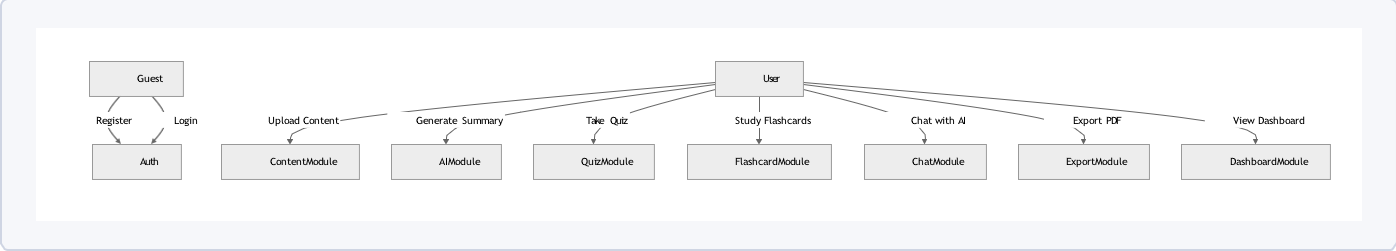
\includegraphics[width=0.9\textwidth]{chapters/chapter05/images/image2.png}
\caption{Use Case Diagram showing interactions between users and system features.}
\label{fig:use_case}
\end{figure}

Because calls to external LLM APIs can take 10--60 seconds, the generation process is handled asynchronously. Figure~\ref{fig:sequence_gen} traces the full sequence: the user submits content from the React frontend, the Go backend creates a job and places it in the Redis queue, a background worker picks up the job and sends requests to the Gemini API, and the results are stored in PostgreSQL. The user is notified via a WebSocket message.

Figure~\ref{fig:auth_matrix} illustrates the authentication flow. It covers the OAuth login process, JWT token signing on the backend, the issuance of secure HttpOnly refresh tokens, and the subsequent token validation that occurs on each authenticated API request.

\begin{figure}[htbp]
\centering
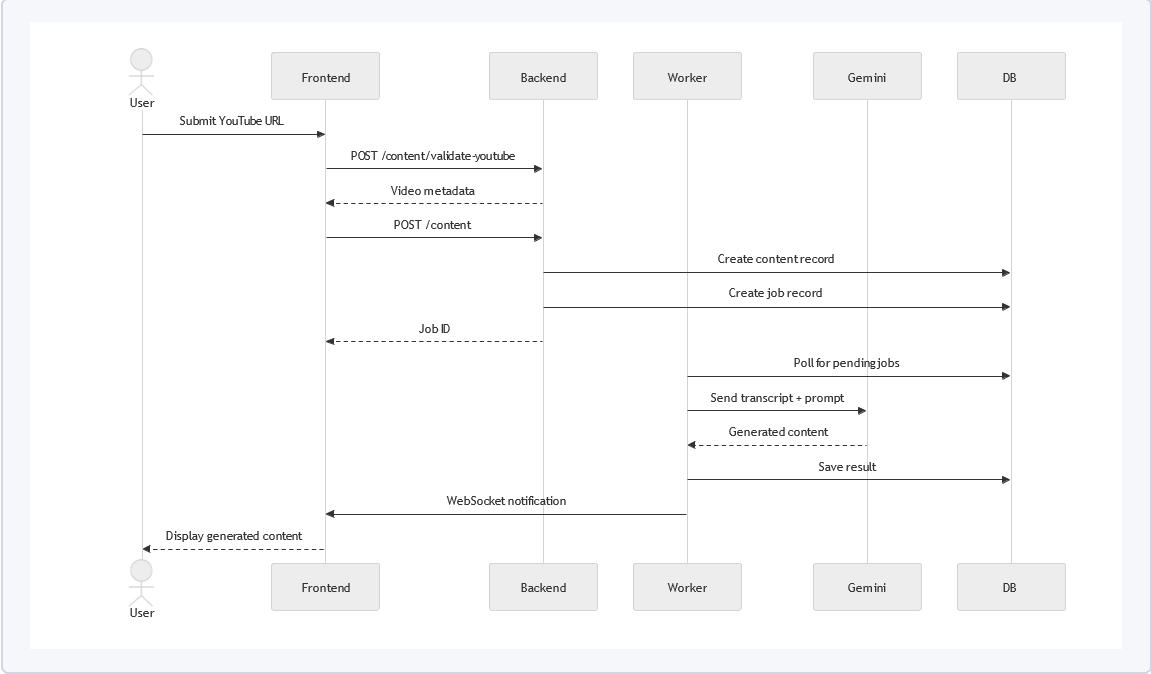
\includegraphics[width=\textwidth]{chapters/chapter05/images/image3.png}
\caption{Sequence Diagram for asynchronous content generation via the LLM API.}
\label{fig:sequence_gen}
\end{figure}

\begin{figure}[htbp]
\centering
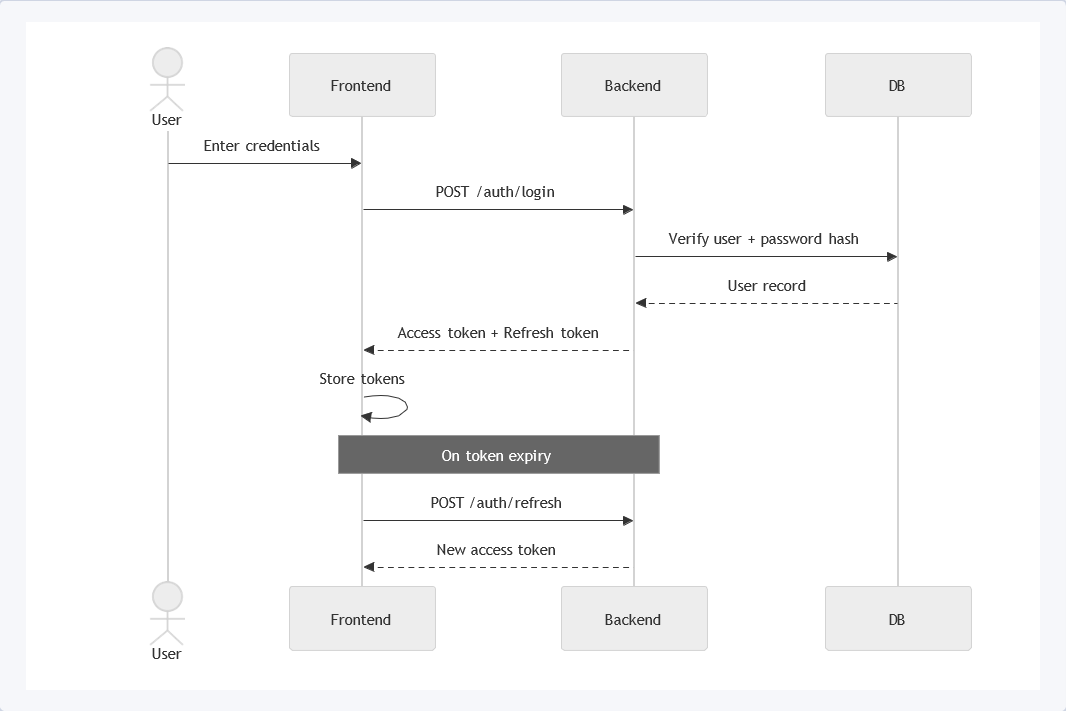
\includegraphics[width=\textwidth]{chapters/chapter05/images/image4.png}
\caption{Sequence Diagram for the JWT-based authentication flow.}
\label{fig:auth_matrix}
\end{figure}

\section{Entity-Relationship Diagram and Database Indexing}
The database structure is shown in Figure~\ref{fig:er_matrix}. It maps the relationships between Users, the extracted Content, and the generated artifacts stored across the Summaries, Quizzes, Presentations, and Flashcards tables. Foreign key constraints enforce referential integrity between these entities.

One key design decision was how to store the variable-structure outputs from the LLM inside a relational database. Rather than creating deeply normalized tables, Lectura stores these outputs in PostgreSQL's JSONB column type, which supports Generalized Inverted Indexes (GIN) for efficient lookups on nested keys. For standard columns like \texttt{created\_at} and \texttt{user\_id}, the system uses B-Tree indexes with logarithmic search time:

\begin{equation}
    T_{\text{search}} \approx O(\log_b n)
\end{equation}

Where $b$ is the branching factor and $n$ is the number of rows. By combining B-Tree indexes on relational columns with GIN indexes on JSONB columns, the database handles both structured queries and flexible AI-generated content efficiently.

\begin{figure}[htbp]
\centering
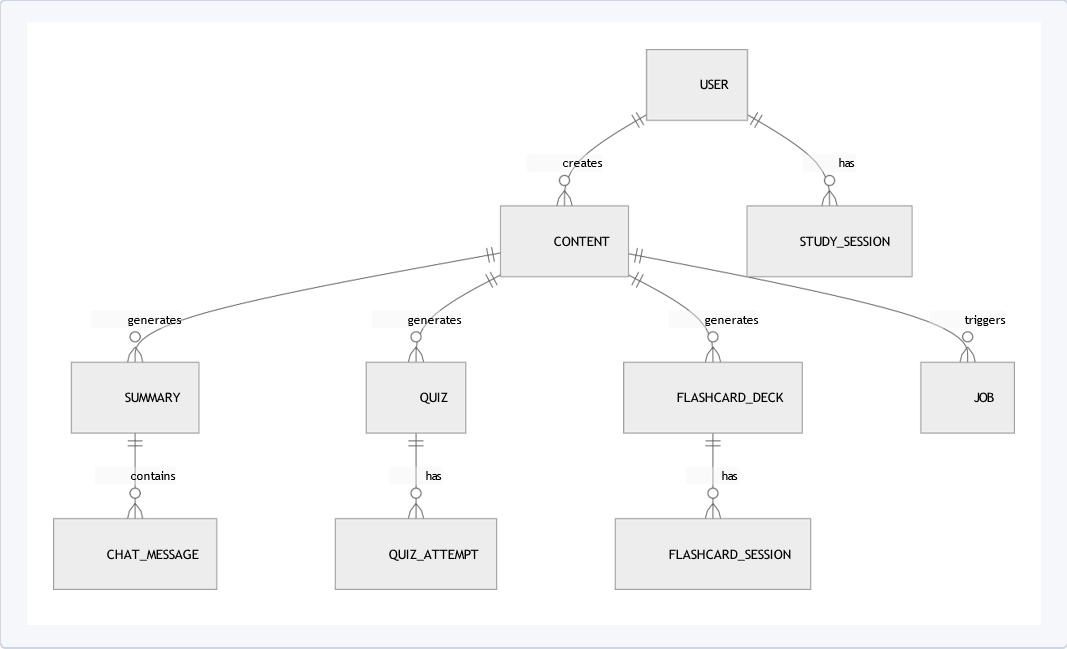
\includegraphics[width=0.9\textwidth]{chapters/chapter05/images/image5.png}
\caption{Entity-Relationship Diagram for the PostgreSQL database schema.}
\label{fig:er_matrix}
\end{figure}

\section{Component Architecture and Worker Pool Design}
On the frontend, separate modules handle authentication, media upload, and artifact rendering independently. On the backend, the Go application follows a layered structure: an API router directs requests to handler functions, which call business logic services, which interact with database repositories. The worker pool operates as a separate subsystem that reads from the job queue independently of the main request-handling thread.

The worker pool is the central mechanism that allows the backend to remain responsive during long-running AI generation tasks. By processing LLM requests in background goroutines, the system can handle many concurrent generation requests without blocking, isolate slow API responses from affecting other users, support automatic retries with exponential backoff, and prevent any single long request from consuming server resources indefinitely.

\section{Technology Stack Justification}
This section justifies the key technology choices made during the development of the Lectura platform.

\subsection{Frontend: React}
Table~\ref{tab:frontend_comparison} compares the main JavaScript/TypeScript frameworks considered.

\begin{table}[htbp]
\centering
\resizebox{\textwidth}{!}{%
\begin{tabular}{|l|p{4cm}|p{4cm}|p{4cm}|}
\hline
\textbf{Criterion} & \textbf{React (Selected)} & \textbf{Vue.js} & \textbf{Angular} \\ \hline
State Management & Flexible (Zustand, Redux, React Query). & Built-in (Pinia). & Standardized (RxJS). \\ \hline
Ecosystem & Very large third-party library ecosystem. & Growing but smaller. & Enterprise-focused. \\ \hline
Rendering & Virtual DOM reconciliation. & Virtual DOM reconciliation. & Incremental DOM updates. \\ \hline
TypeScript Support & Full TypeScript integration. & Excellent native support. & TypeScript required. \\ \hline
\end{tabular}%
}
\vspace{6pt}
\caption{Comparison of frontend SPA frameworks.}
\label{tab:frontend_comparison}
\end{table}

React 18 was selected primarily for its modular component architecture and mature ecosystem. The project required rendering dynamic content types — including mathematical LaTeX notation in quizzes and generated Markdown tables — and React's declarative model makes it straightforward to integrate specialized rendering libraries. React Query was used to handle server-state caching, preventing unnecessary network requests.

\subsection{Backend: Go}
Table~\ref{tab:backend_comparison} compares the three main backend candidates.

\begin{table}[htbp]
\centering
\resizebox{\textwidth}{!}{%
\begin{tabular}{|l|p{4cm}|p{4cm}|p{4cm}|}
\hline
\textbf{Criterion} & \textbf{Go (Selected)} & \textbf{Node.js (TypeScript)} & \textbf{Python (FastAPI)} \\ \hline
Concurrency Model & Native goroutines with precise memory control. & Single-threaded event loop. & Threading / AsyncIO (limited by GIL). \\ \hline
Execution Speed & Very high (compiled to native binary). & High (JIT compilation via V8). & Moderate (interpreted). \\ \hline
Memory Usage & Low. & Moderate to high. & High. \\ \hline
Type Safety & Strict, enforced at compile time. & Optional (TypeScript). & Runtime type hints only. \\ \hline
\end{tabular}%
}
\vspace{6pt}
\caption{Backend language comparison for concurrent workload handling.}
\label{tab:backend_comparison}
\end{table}

Go was chosen because the Lectura architecture relies heavily on a Worker Pool pattern to handle LLM generation tasks that can take 10--60 seconds each. Go's goroutines and channel-based communication provide an efficient way to manage many concurrent tasks with low memory overhead.

\subsection{Database: PostgreSQL}
PostgreSQL was chosen because it handles both structured relational data (user accounts, authentication) and flexible AI-generated content (via JSONB columns) without requiring two separate databases.

\begin{table}[htbp]
\centering
\resizebox{\textwidth}{!}{%
\begin{tabular}{|l|p{4.5cm}|p{3.5cm}|p{3.5cm}|}
\hline
\textbf{Criterion} & \textbf{PostgreSQL (Selected)} & \textbf{MongoDB} & \textbf{MySQL} \\ \hline
Data Integrity & Full ACID compliance. & Eventually consistent. & ACID compliant. \\ \hline
Schema Flexibility & Strong (JSONB with indexing). & Native document store. & Limited. \\ \hline
Query Capabilities & Advanced (array ops, CTEs, window functions). & Good for document queries. & Standard SQL. \\ \hline
Complex Joins & Well optimized. & Poor performance. & Well optimized. \\ \hline
\end{tabular}%
}
\vspace{6pt}
\caption{Database comparison based on schema flexibility and query performance.}
\label{tab:database_comparison}
\end{table}

\subsection{LLM Provider: Google Gemini}
Google Gemini 3 Flash was selected primarily for its large context window. In an educational application where the input might be a full lecture transcript, smaller context windows would require implementing a RAG pipeline with vector embeddings — adding significant complexity. Gemini's million-token window allows the system to pass the entire source document in a single API call. Its lower cost per token and fast response times also make it practical for a student-facing application.

\begin{table}[htbp]
\centering
\resizebox{\textwidth}{!}{%
\begin{tabular}{|l|p{4cm}|p{4cm}|p{4cm}|}
\hline
\textbf{Criterion} & \textbf{Google Gemini 3 Flash} & \textbf{OpenAI GPT-4o} & \textbf{Anthropic Claude 3.5} \\ \hline
Context Window & 1+ million tokens. & 128,000 tokens. & 200,000 tokens. \\ \hline
Response Speed & Very fast. & Moderate. & Moderate. \\ \hline
Cost & Low. & High. & High. \\ \hline
Format Compliance & Good. & Excellent. & Very good. \\ \hline
\end{tabular}%
}
\vspace{6pt}
\caption{Comparison of LLM providers by context window, speed, and cost.}
\label{tab:llm_comparison}
\end{table}

\subsection{Document Export: Puppeteer}
\begin{table}[htbp]
\centering
\resizebox{\textwidth}{!}{%
\begin{tabular}{|l|p{4cm}|p{4cm}|p{4cm}|}
\hline
\textbf{Criterion} & \textbf{md-to-pdf (Puppeteer)} & \textbf{jsPDF} & \textbf{pdfmake} \\ \hline
Execution & Server-side headless browser. & Client-side Canvas API. & Client-side JSON-based. \\ \hline
Layout Support & Full CSS/HTML rendering. & Manual coordinate positioning. & Abstract layout definitions. \\ \hline
Math Rendering & Full support via browser engine. & Very limited. & Very limited. \\ \hline
\end{tabular}%
}
\vspace{6pt}
\caption{Comparison of PDF export methods.}
\label{tab:export_comparison}
\end{table}

Server-side rendering using a headless Chromium instance (via Puppeteer) was selected because client-side libraries struggle with complex layouts and mathematical notation. The backend maintains a pool of pre-started Chromium instances with defined memory limits. The total memory usage $M_{\text{total}}$ for $n$ concurrent exports is bounded by:

\begin{equation}
    M_{\text{total}}(n) = M_{\text{base}} + n \times (M_{\text{instance}} + M_{\text{content}})
\end{equation}

After processing a threshold of $k$ documents, each instance is terminated and replaced to prevent memory leaks. This recycling approach keeps memory usage predictable even during high-traffic periods.